\documentclass{article}
\usepackage{graphicx}
\usepackage[utf8x]{inputenc}
\usepackage[russian]{babel}

\usepackage[a4paper,body={6.5in, 9.7in}]{geometry}
\usepackage{amssymb,amsmath}
\begin{document}
\thispagestyle{empty}
\begin{itemize}
\item $M$ : масса каретки %masse du chariot
\item $f$ : сила, приложенная мотором %force appliquée par le moteur
\item $m$ : масса маятника %masse du bras
\item $2l$ : длина маятника ($l$ - расстояние между осью и цетром масс) %longueur du bras ($l$ etant la distance entre le pivot et le centre de gravité)
\item $I$ : момент инерции маятника %moment d'inertie du bras (pour notre bras il est égal à $\frac{m(2l)^2}{3}$
\item $\theta(t)$ : угол между маятником и вертикалью, увеличивется в направлении часовой стрелки %angle entre le bras et la verticale, zero pour la position verticale, increment en clockwise
\item $x(t)$ : координата каретки %coordonnée du chariot, increment à droite
\end{itemize}

\centerline{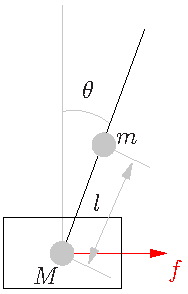
\includegraphics[width=.3\linewidth]{schema.pdf}}



%2eme lois de Newton sur le chariot :
Второй закон Ньютона для каретки:
\begin{align*}
M\ddot{x} & = f - m\frac{d^2}{dt^2}(x + l\sin(\theta)) = \\
          & = f - m\frac{d}{dt}(\dot{x} + l\dot{\theta}\cos(\theta)) = \\
          & = f - m(\ddot{x} + l\ddot{\theta}\cos(\theta) - l\left(\dot{\theta}\right)^2\sin(\theta))
\end{align*}


%Linearisation autours de $\theta=0$
Линеаризуем вокруг $\theta=0$
$$
\left \{ \begin{array}{r l}
\sin(\theta) & \approx \theta \\
\cos(\theta) & \approx 1      \\
\left(\dot{\theta}\right)^2 & \approx 0
\end{array} \right.
$$


\begin{equation}
(M+m)\ddot{x} + ml\ddot{\theta} \approx f
\end{equation}


%2eme lois de Newton (version rotationnelle) pour le bras :
Второй закон Ньютона (вращательная версия) для маятника:
\begin{align*}
I\ddot{\theta} & = lmg\sin(\theta) - lm\cos(\theta)\frac{d^2}{dt^2}(x + l\sin(\theta)) + lm\sin(\theta)\frac{d^2}{dt^2}(l\cos(\theta)) = \\
               & = lmg\sin(\theta) - lm\cos(\theta)\left(\ddot{x} + l\ddot{\theta}\cos(\theta) - l\left(\dot{\theta}\right)^2\sin(\theta)\right) + lm\sin(\theta)\left(-l\ddot{\theta}\sin(\theta) - l\left(\dot{\theta}\right)^2\cos(\theta) \right) = \\
               & = lmg\sin(\theta) - lm\cos(\theta)\ddot{x} - l^2m\ddot{\theta}
\end{align*}

%Pareil, linearisons l'equation:
Опять же, линеаризуем:

\begin{equation}
lm\ddot{x} + (I+ml^2)\ddot{\theta} \approx lmg \theta
\end{equation}


%Ecrivons les équations (1) + (2) dans un système lineaire :
Запишем уравнения (1) и (2) в систему:
$$
\begin{bmatrix}M+m & ml \\ ml & I+ml^2\end{bmatrix}\begin{bmatrix}\ddot{x}\\ \ddot{\theta}\end{bmatrix} = \begin{bmatrix}f\\ lmg\theta\end{bmatrix}
$$

$$
\Rightarrow\begin{bmatrix}\ddot{x}\\ \ddot{\theta}\end{bmatrix} = \begin{bmatrix}M+m & ml \\ ml & I+ml^2\end{bmatrix}^{-1}\begin{bmatrix}f\\ lmg\theta\end{bmatrix}
$$



%Pour l'instant pour simplifier appelons le determinant de la matrice $D$ :
Назовём для удобства детерминант буквой $D$:

$$
D = \begin{vmatrix}M+m & ml \\ ml & I+ml^2\end{vmatrix} = (I+ml^2)(M+m) - m^2l^2
$$

%L'inverse de matrice 2x2 est simple à calculer :
Обратим матрицу:

$$
\Rightarrow\begin{bmatrix}\ddot{x}\\ \ddot{\theta}\end{bmatrix} = \frac{1}{D}\begin{bmatrix}I+ml^2 & -ml \\ -ml & m+M\end{bmatrix}\begin{bmatrix}f\\ lmg\theta\end{bmatrix}
$$


%Facile à écrire le systeme des equadiffs lineaires (version continue) :
Переписываем систему линейных диффуров:

$$
\begin{bmatrix}\dot{x}\\\ddot{x}\\\dot{\theta}\\\ddot{\theta}\end{bmatrix} = 
\begin{bmatrix}
0 & 1 & 0 & 0\\
0 & 0 & \frac{-l^2m^2g}{D} & 0 \\ 
0 & 0 & 0 & 1\\
0 & 0 & \frac{lmg(M+m)}{D} & 0
\end{bmatrix}
\begin{bmatrix}{x}\\\dot{x}\\{\theta}\\\dot{\theta}\end{bmatrix}  +
\begin{bmatrix} 0 \\ \frac{I+ml^2}{D} \\ 0 \\ \frac{-lm}{D} \end{bmatrix} f
$$


%Maintenant il serait le temps de discretiser, on a en continu ($\vec{x}$ c'est bien le vecteur 4D de nos états, $A$ une matrice 4x4, $B$ une matrice 4x1, la ligne precedente, quoi) :
Теперь дискретизация непрерывных диффуров:
$$
\dot{\vec{x}}(t) = A \vec{x}(t) + Bf(t)
$$

%Pour le pas constant $\Delta t$ on a la relation suivante :
Для постоянного шага $\Delta t$ получаем:

$$
\vec{x}((k+1)\Delta t) \approx \vec{x}(k\Delta t) + \Delta t \dot{\vec{x}}(k\Delta t)
$$

$$
\Rightarrow \vec{x}_{k+1} \approx \vec{x}_k + \Delta t (A\vec{x}_k + B f_k)
$$

%Appelons la matrice identité 4x4 $E$ :
$E$ - единичная матрица 4x4:

$$
\Rightarrow \vec{x}_{k+1} \approx (E+\Delta t A) \vec{x}_k + \Delta t B f_k
$$


%Bon, maintenant pour notre bras on sais calculer le moment d'inertie:
Поскольку момент инерции нам известен, упрощаем выражение:
$$
I = \frac{4}{3} m l^2 \Rightarrow D = \frac{l^2m}{3}(7M + 4m)
$$

$$
\vec{x}_{k+1} = \begin{bmatrix}1 & \Delta t & 0 & 0 \\ 0 & 1 & -\frac{3mg\Delta t}{7M+4m} & 0 \\ 0 & 0 & 1 & \Delta t \\ 0 & 0 & \frac{3g(m+M)\Delta t}{l(7M+4m)} & 1\end{bmatrix} \vec{x}_k + \begin{bmatrix}0 \\ \frac{7 \Delta t}{7M+4m} \\ 0 \\ \frac{-3\Delta t}{l(7M+4m)}\end{bmatrix} f_k
$$


\end{document}


